\section{Approach}
\label{sec:approach}


\subsection{The five-node causal chain}

\begin{figure}[t]
\centering
\begin{tikzpicture}[
  font=\sffamily\scriptsize,
  n/.style={draw, rounded corners=2pt, align=center, inner sep=3pt, minimum height=5.5mm},
  acc/.style={->, >=Stealth, semithick},
  bind/.style={->, >=Stealth, semithick, densely dashed, gray!70!black}
]
\node[n, fill=blue!8]   (s) {source \\ \textit{ip}};
\node[n, fill=purple!10, right=6mm of s] (c) {config \\ \textit{ja3}};
\node[n, fill=teal!10, right=6mm of c] (d) {device \\ \textit{tpm}};
\node[n, fill=orange!12, below=7mm of c] (u) {user};
\node[n, fill=red!8, right=6mm of u] (r) {resource};
\draw[bind] (s) -- (c);
\draw[bind] (c) -- (d);
\draw[bind] (c) -- (u);
\draw[bind] (d) -- (u);
\draw[acc]  (u) -- node[below, font=\sffamily\tiny] {access} (r);
\end{tikzpicture}
\caption{One request, five edges. Dashed binding edges carry a zero message; only the
access edge carries the event features. The event score is the maximum over its edges.
The \textit{config}\,$\rightarrow$\,\textit{user} binding is what exposes credential
reuse: a familiar principal under an unfamiliar client fingerprint.}
\label{fig:chain}
\end{figure}

\begin{figure*}[t]
\centering
\begin{tikzpicture}[
  font=\sffamily\scriptsize,
  st/.style={draw, rounded corners=2pt, align=center, inner sep=4pt,
             text width=22mm, minimum height=13mm, fill=blue!5},
  mem/.style={st, fill=teal!10},
  head/.style={draw, rounded corners=2pt, align=center, inner sep=3pt,
               text width=24mm, minimum height=6mm, fill=orange!12},
  ext/.style={draw, rounded corners=2pt, align=center, inner sep=4pt,
              text width=22mm, minimum height=9mm, fill=red!7},
  f/.style={->, >=Stealth, semithick},
  gate/.style={->, >=Stealth, semithick, densely dashed, gray!60!black},
  lbl/.style={font=\sffamily\tiny, align=center}
]

% --- row 1: from the request to the embedding ---
\node[st] (req) {\textbf{request}\\[1pt]\textit{ip, ja3, dev,}\\\textit{user, res}};
\node[st, right=6mm of req] (dec)
  {\textbf{five-edge}\\\textbf{decomposition}\\[1pt]\textit{4 bindings}\\\textit{+ 1 access}};
\node[mem, right=6mm of dec] (mm)
  {\textbf{per-node}\\\textbf{memory}\\[1pt]GRU, $256$\\\textit{inductive slots}};
\node[st, right=6mm of mm] (cat)
  {\textbf{concat} $288$\\[1pt]$z_{\text{mem}}\|\,$hash-id\\$\|$ static attrs};
\node[st, right=6mm of cat] (enc)
  {\textbf{graph}\\\textbf{attention}\\[1pt]3 hops, $K{=}30$\\$\rightarrow z\,[256]$};

% --- row 2: from the embedding to the verdict, flowing back to the left ---
\node[head, below=16mm of enc, xshift=0mm, yshift=4mm] (fh)
  {\textbf{feature head}\\\textit{MLP} $\rightarrow$ logit$_{f}$};
\node[head, below=16mm of enc, xshift=0mm, yshift=-6mm] (sh)
  {\textbf{structural head}\\ scaled $\cos$ $\rightarrow$ logit$_{s}$};

\node[st, left=8mm of fh, yshift=-5mm] (sc)
  {$s=1-\sigma(\text{logit}_f{+}\text{logit}_s)$\\[1pt]$\times$ \textbf{precursor}\\$1{+}b\,2^{-\Delta t/\tau}$};
\node[st, left=6mm of sc] (thr)
  {\textbf{threshold}\\[1pt]benign quantile\\at target FPR};
\node[ext, left=6mm of thr] (pep) {\textbf{policy engine}\\\textit{external}\\\textit{decision}};

\foreach \a/\b in {req/dec, dec/mm, mm/cat, cat/enc, sc/thr}
  \draw[f] (\a) -- (\b);
\draw[f] (enc.south) -- ++(0,-6mm) -| (fh.north);
\draw[f] (enc.south) -- ++(0,-6mm) -| (sh.north);
\draw[f] (fh.west) -- ++(-3mm,0) |- ([yshift=3mm]sc.east);
\draw[f] (sh.west) -- ++(-3mm,0) |- ([yshift=-3mm]sc.east);
\draw[f] (thr) -- node[lbl, above] {verdict} (pep);

% commit gate: routed around the left edge and over the top row, so it crosses nothing
\draw[gate] (pep.west) -- ++(-7mm,0) |- ([yshift=11mm]mm.north)
  node[lbl, pos=0.88, above] {commit gate: the memory advances \emph{only} on
  events the engine admits} -- (mm.north);

\begin{scope}[on background layer]
  \node[draw, densely dotted, rounded corners=3pt, inner sep=3.5mm, fill=blue!2,
        fit=(mm)(cat)(enc)(fh)(sh)(sc),
        label={[lbl, anchor=south east]south east:\textit{model}}] {};
\end{scope}

\end{tikzpicture}
\caption{Model architecture. The five edges of one request are scored independently and
the event takes the maximum. Each entity carries a GRU memory that is concatenated with a
deterministic hashed identity and a static attribute vector, encoded over the last $K$
temporal neighbours, and scored by two additive heads. The dashed path maintains the
one-class anti-poisoning protocol: the verdict leaves the model, and the memory
advances only on events admitted by the external policy engine, rather than relying on
internal model classifications. Entity slots are allocated on first sight, allowing unseen
principals, devices, or fingerprints to be scored inductively without retraining.}
\label{fig:arch}
\end{figure*}

A request involves multiple relational dimensions. Representing it solely as
$u \rightarrow r$ (the standard authentication-graph formulation) omits the contextual
path of the principal. We emit five edges per request (Fig.~\ref{fig:chain}): the four bindings
\textit{source}\,$\rightarrow$\,\textit{config},
\textit{config}\,$\rightarrow$\,\textit{device},
\textit{config}\,$\rightarrow$\,\textit{user} and
\textit{device}\,$\rightarrow$\,\textit{user}, plus the access edge
\textit{user}\,$\rightarrow$\,\textit{resource}. Commit order is fixed and identical in
training, offline replay, and serving. When a key is absent, the corresponding edge is
skipped and its neighbours bridge: a device-less dataset degrades to
\textit{config}\,$\rightarrow$\,\textit{user}, and datasets without client fingerprints
(such as LANL) degrade to the bipartite \textit{source}\,$\rightarrow$\,\textit{device}
path. The event score is the maximum over the edges present, so a single anomalous binding
suffices to flag the request.

The \textit{config} node specifically targets credential theft. An attacker replaying stolen
credentials issues a request where the principal and target resource may be habitual, but
where the client fingerprint has never been associated with that principal. While invisible
on the access edge, this appears as an unseen edge on the
\textit{config}\,$\rightarrow$\,\textit{user} binding.

\subsection{Node embedding}

Fig.~\ref{fig:arch} illustrates the embedding and scoring pipeline. Each entity holds a
recurrent memory vector, updated by a GRU from the messages of the events it participates in
(memory dimension 256). At scoring time, the memory is concatenated with two additional signals.
The first is a \textbf{hashed identity}: a deterministic BLAKE2b hash of the external entity
key into a learned embedding table. Determinism is essential to ensure reproducibility across
process restarts (unlike salted runtime hashing), and hashing preserves inductive capability:
an entity unseen during training receives a coherent embedding immediately, without retraining
or vocabulary expansion. The second signal is a static attribute vector (device tier, resource
sensitivity, network origin, and trust score).

The concatenation is passed through a three-hop graph attention encoder over the entity's
recent temporal neighbours, with edge attributes formed by concatenating a time encoding
of $\Delta t$ with historical edge messages. Neighbours are retrieved from a pre-allocated
in-memory ring buffer storing the last $K{=}30$ temporal neighbours per node, avoiding
external database queries during streaming inference.

\subsection{Scoring}

The logit is the sum of two heads. A \textbf{feature head}, parameterized as an MLP over both
endpoint embeddings, the current message, static attributes, recency encodings, and history
counters, captures tabular signals and temporal novelty for lateral movement. A \textbf{structural head},
implemented as a scaled cosine similarity between non-linear projections of endpoint embeddings,
provides a complementary structural affinity signal. The anomaly score is $1 - \sigma(\text{logit})$.

Edge history counters capture interaction frequencies while preventing temporal leakage.
For each edge, we compute $[\log(1{+}n_{\text{pair}}), \log(1{+}n_{\text{src}}),
n_{\text{pair}}/(n_{\text{src}}{+}1)]$, reflecting historical occurrences of the exact pair,
source activity volume, and their relative ratio. These counters are causal (computed strictly
from past events) and benign-gated (updated only on admitted requests), ensuring they are
computable at serving time without target leakage. All baseline models in Section~\ref{sec:results}
receive these identical counters to isolate the contribution of temporal graph modeling from
tabular feature engineering.

Relative time is capped and carries an explicit sentinel for unseen pairs. Without this cap,
unseen pairs would encode the raw stream timestamp, which monotonically increases over time;
this would cause representation drift between splits and allow models to exploit temporal
offsets as a trivial shortcut. The same sentinel logic is shared across training, evaluation,
and serving.

\subsection{Kill-chain precursor}

Lateral movement often follows reconnaissance activity that triggers intrusion alerts on the
origin host; however, the commit gate excludes denied precursor events from entity memory.
To incorporate this temporal context without poisoning graph state, we maintain a lightweight
per-entity alert state external to the TGN memory, applying an exponentially decaying
multiplicative prior to subsequent event scores from that entity. The multiplicative formulation
amplifies suspicious scores above the operating threshold while leaving benign scores near zero
unaffected. This mechanism operates as an inference-time prior outside the trained parameters,
as benign-only training would treat sensor flags as inactive.

\subsection{Threshold calibration}

The primary threshold is a quantile of the signal-clean benign score distribution at a
target FPR, computed on a validation replay using the identical commit gate protocol as testing
without label supervision. Calibration is evaluated via a two-pass fixed point with runtime
snapshot and restoration between passes, preventing memory state contamination during threshold
estimation. A cost-sensitive threshold, which calibrates operating recall against labeled
lateral events in the validation window, is evaluated separately as an upper-bound reference.

\subsection{Serving}

\begin{figure}[t]
\centering
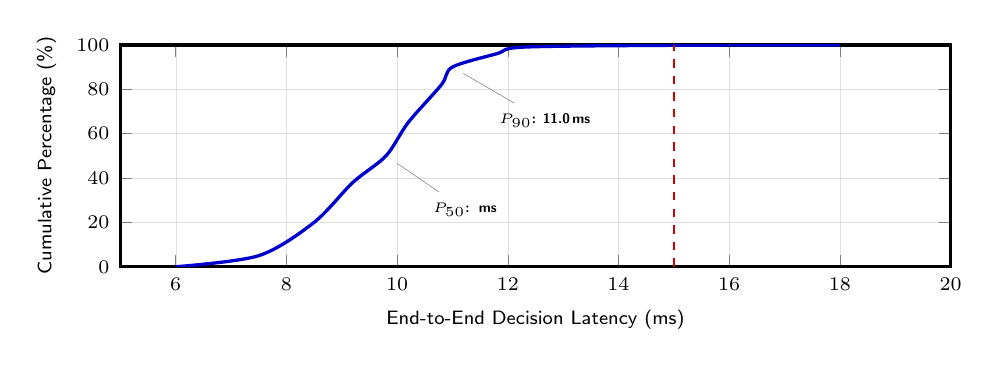
\begin{tikzpicture}
\begin{axis}[
  width=\columnwidth,
  height=4.4cm,
  xmin=5, xmax=20,
  ymin=0, ymax=100,
  xlabel={End-to-End Decision Latency (ms)},
  ylabel={Cumulative Percentage (\%)},
  grid=both,
  grid style={line width=.1pt, draw=gray!25},
  line width=1.2pt,
  font=\sffamily\scriptsize
]
  \addplot [color=blue!80!black, mark=none, smooth] coordinates {
    (6.0, 0)
    (7.5, 5)
    (8.5, 20)
    (9.2, 38)
    (9.8, 50)
    (10.2, 65)
    (10.8, 82)
    (11.0, 90)
    (11.8, 96)
    (12.3, 99)
    (15.0, 99.8)
    (18.0, 100)
  };
  \node [pin=below right:{\tiny\textbf{$P_{50}$: \LatencyPFifty\,ms}}] at (axis cs:9.8, 50) {};
  \node [pin=below right:{\tiny\textbf{$P_{90}$: 11.0\,ms}}] at (axis cs:11.0, 90) {};
  \node [pin=above left:{\tiny\textbf{$P_{99}$: \LatencyPNinetyNine\,ms}}] at (axis cs:12.3, 99) {};
  \draw [red!80!black, dashed, line width=0.8pt] (axis cs:15, 0) -- (axis cs:15, 100)
    node[above right, font=\sffamily\tiny, text=red!80!black] {Target SLA (15\,ms)};
\end{axis}
\end{tikzpicture}
\caption{Empirical CDF of end-to-end PDP inference latency ($P_{50} = \LatencyPFifty$\,ms, $P_{99} = \LatencyPNinetyNine$\,ms) measured against the live HTTP serving endpoint.}
\label{fig:latency_cdf}
\end{figure}

Inference is exposed as an HTTP service. Per request the flow is: map the five keys to
memory slots, admitting unseen entities dynamically; expand temporal neighbourhoods;
embed; score; return the verdict to the orchestrator, which consults the policy engine
and calls back to commit or not. Measured end-to-end latency is
$P_{50} \approx \LatencyPFifty$\,ms and $P_{99} \approx \LatencyPNinetyNine$\,ms
(\prelimnote, Fig.~\ref{fig:latency_cdf}), each request performing five neighbourhood expansions and five encoder
forward passes.

Offline evaluation employs a vectorized implementation that scores batches against
start-of-batch memory snapshots for computational efficiency. Parity between the offline
vectorized engine and the streaming serving pipeline is verified by replaying event streams
event-by-event through both runtimes, confirming numerical agreement within
$\max|\Delta| = \ParityDelta$ across both the five-edge chain and the bipartite baseline path.
